%=== CHAPTER THREE (3) ===
%=== (Actual work done and contribution, including literature survey) ===

\chapter{Typical Approaches}
\begin{spacing}{1.5}
\setlength{\parskip}{0.3in}

There are several methods we see today for chip interconnects, such as the MCM method which integrates and interconnects multiple standard ASIC components on a package substrate, the 2.5D package method which integrates ASIC components on a Si or interposer layer (organic material doping), including die-to-die connections between two or more die via an interposer layer. stacking and interconnecting in the z-axis dimension. For commercialization, there should be three options from the EDA provider's point of view: hardcore IP, softcore IP, and Chiplet. The third option is a process that allows Fabless to place the bought hardcore IP on the intermediary layer, laminate or stack it and then interconnect it.

Referring to AMD's previous EPYC processor release: the introduction of the MCM approach to EPYC processor design will require 10\% more wafer area than a single die for I/O communication/connection function blocks between bare dies (D2D), redundant logic, and other additional features. In the end, however, the overall processor chip cost is still 41\% less than a single-die processor, and as individual die sizes and densities are scaled up, future yields could steadily exceed those of single-die.

The so-called multi-chip module MCM is a chip module constructed by directly adhering and interconnecting multiple bare chips on various material substrates composed of conductor layers and dielectric layers. In another word, it is incorporating a module composed of multiple chips into one package. The chips may be ICs, diodes, transistors, MOSFETs, or other active components. The point is that all of them are enclosed in the same package.

The term \textit{MCM} is currently overused. Here we would like to give a definition of MCM for classification. If we look at the packaging category based on the electronic component evolution cycle, we can find that packaging one component is called \textit{packaging}, and packaging multiple components is called \textit{multi-chip package} (MCP). When a part of the circuit or a module is packaged, it is called a multi-chip module package (MCM). The main difference between MCP and MCM is whether it is a complete circuit. MCP has only active components, while MCM includes active components and passive components. 

\begin{figure}[ht]
	\centering
	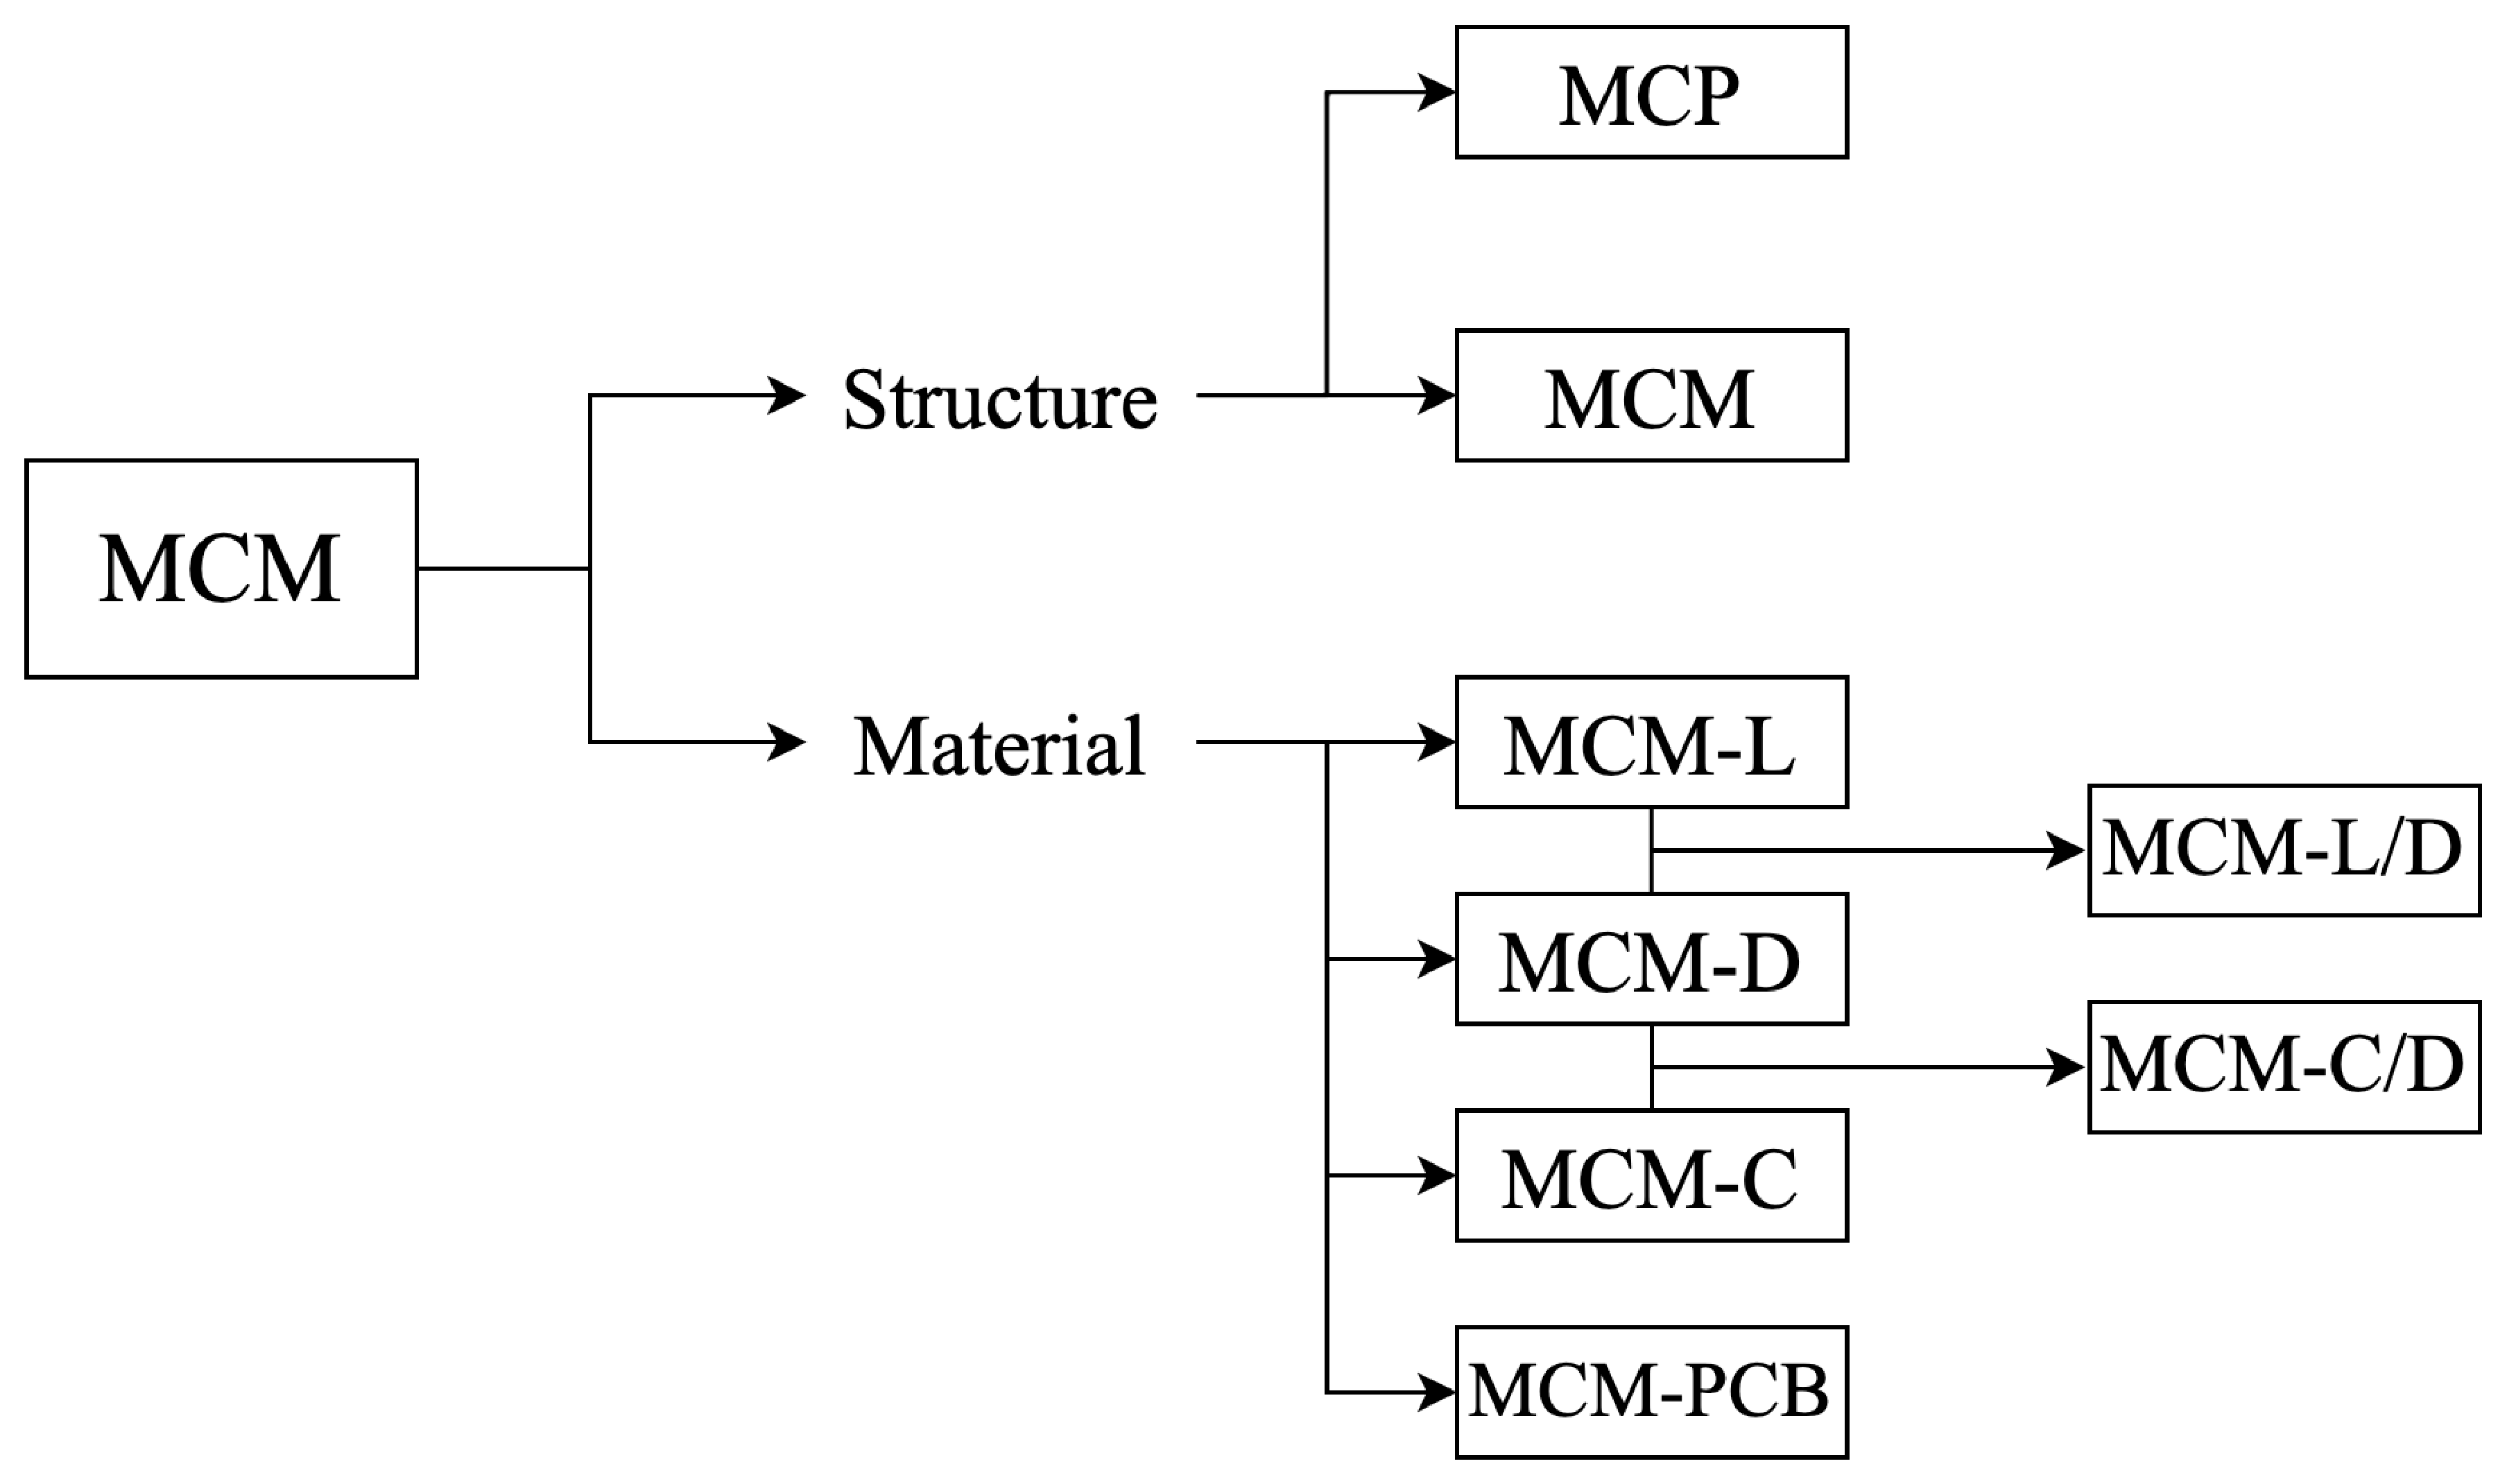
\includegraphics[width=4in, fbox]{Chapter3/mcm1(1).eps}
	\caption{Illustration of MCM categories.}
	\label{fig:chpt3.1} 
\end{figure}

According to different materials and processes, we can divide MCM into four main categories \autoref{fig:chpt3.1}. 

\section{MCM-L (Laminated) and MCM-L/D}

The circuit wires and contacts are formed by deposition or etching on the low temperature co-fired ceramic sheet or metal sheet. Then chips, transistors, and other active components and passive components such as resistors and capacitors are bonded. In order to improve the buried density, it can be combined with MCM-D (so-called MCM-L/D) to achieve higher density by deposition. 

\begin{figure}[ht]
	\centering
	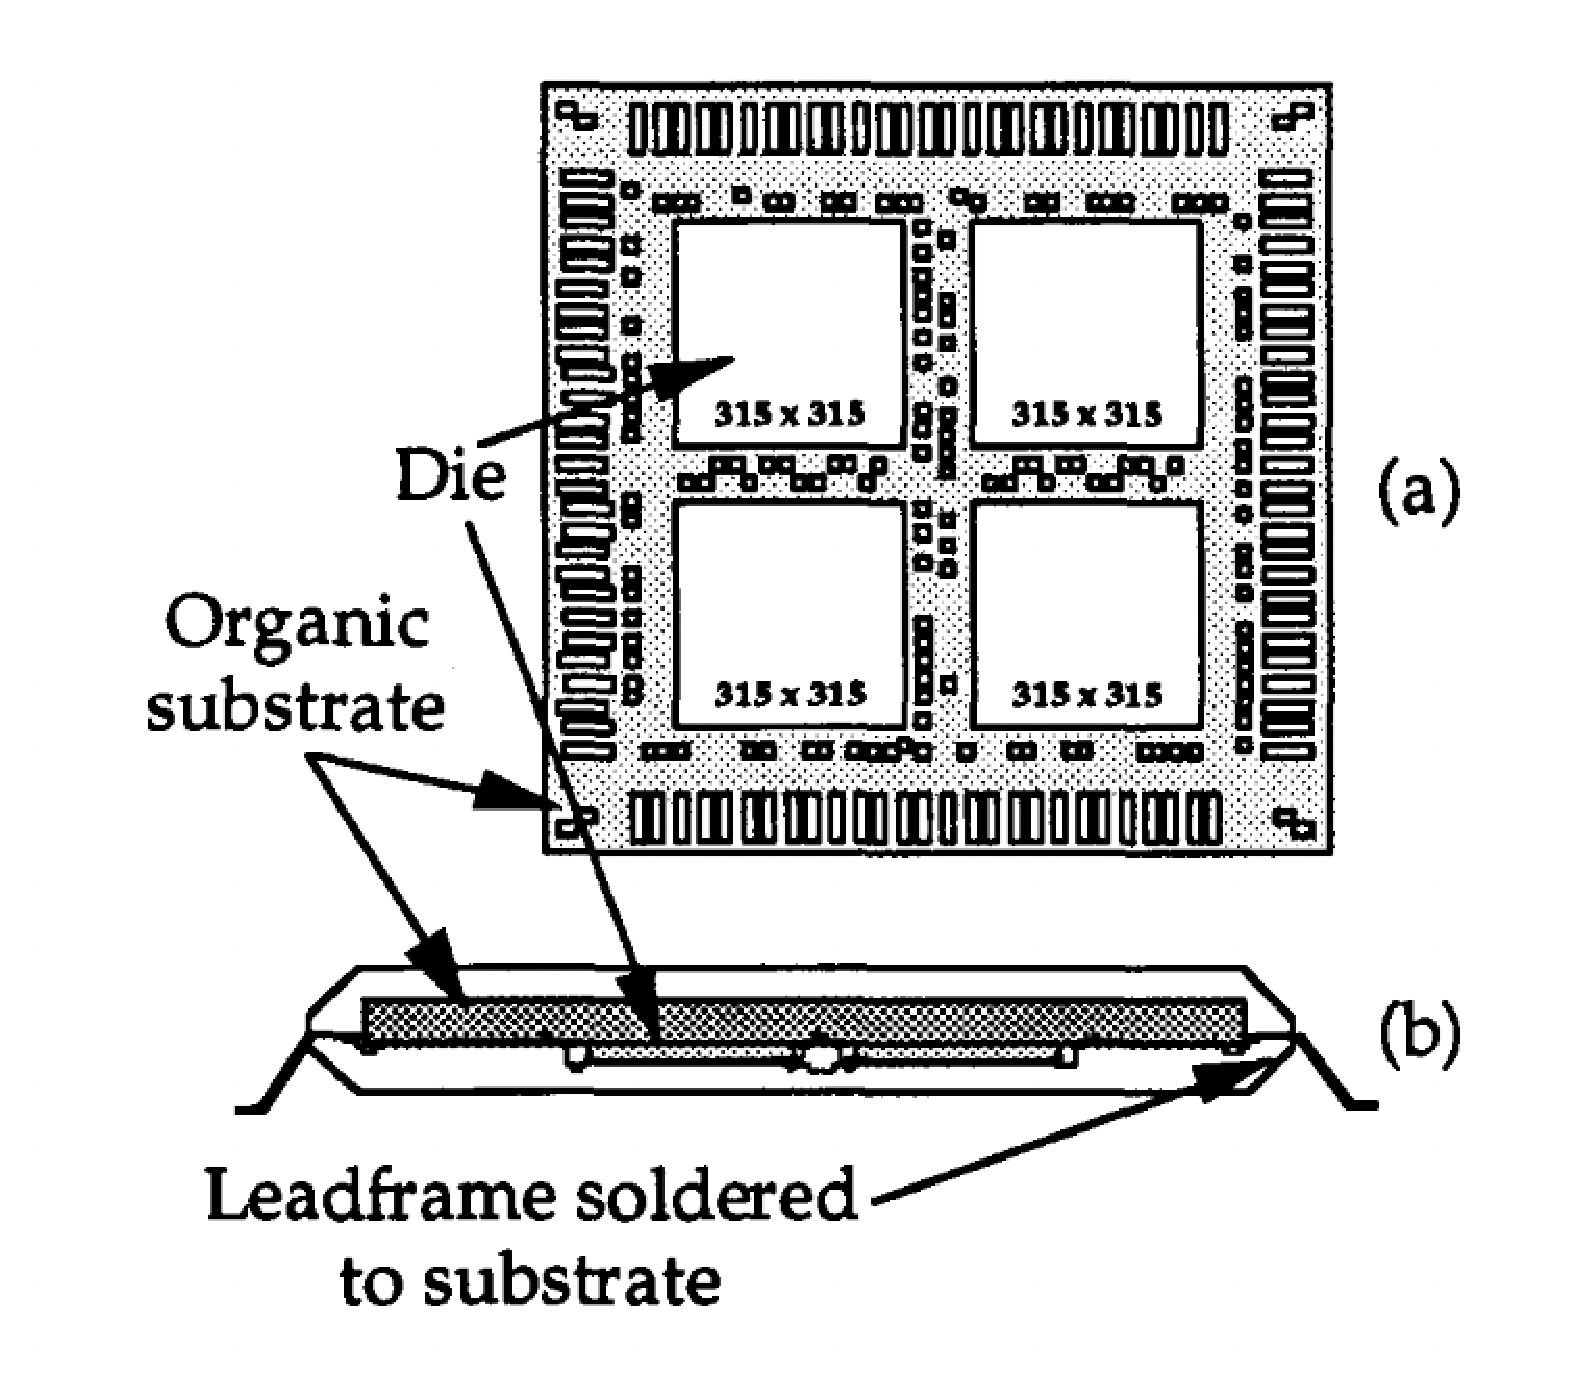
\includegraphics[width=4in, fbox]{Chapter3/2.eps}
	\caption{Schematic of MCM-L packaging of four chips.(Ref. \cite{nachnani1993low}, Fig. 4 )}
	\label{fig:chpt3.2} 
\end{figure}

The development of MCM-L involves evolutionary technological advances to reduce interconnects and vias. From the perspective of cost, it is best to use traditional PWB technology for MCM-L manufacturing. However, this becomes more and more difficult because they need a higher interconnect density of multichip modules continues. Since MCM technology is being considered for the application of mass consumer products, it is very important to focus on controlling the cost of high-density MCM-L. The most important characteristic of evaluating MCM-L technology is the packaging efficiency which is given below.

\begin{equation}
	Packaging\ efficiency(\%)=\frac{Silicon\ chip\ area}{Package\ area}
\end{equation}

\section{MCM-C (Ceramic), MCM-C/D}

It is based on a multilayer ceramic substrate. This method forms wires and contacts in different layers, then, bonds IC, transistors, and other active components, and resistors, resistors, and passive components such as capacitors. In order to increase the buried density, it can be combined with MCM-D (so-called MCM-C/D) to achieve higher density by deposition. MCM-C mainly uses thick film technology (such as combustible metal) to form conductive patterns. It is completely composed of ceramic or glass-ceramic materials, or other materials with a dielectric constant higher than 5. In short, MCM-C is constructed on ceramic or glass-ceramic substrates. The advantages of MCM-C are more wiring layers, wiring density, packaging efficiency, and performance are higher, mainly used for high-reliability products with operating frequency (30-50) MHz.

These ceramics, along with alumina, are fired at high temperatures and require refractory metallization systems, such as tungsten and molybdenum metals. Ceramics fired at temperatures below 1000 ° C can also be used. Low-temperature co-fired ceramics (LTCC) are mainly composed of borosilicate glass systems with gold or silver metallization. MTCC is a new ceramic packaging material system, which uses copper metallization to realize low resistance wiring. These glass-ceramic MCM-C materials show excellent conductivity and good dielectric properties for high-speed transmission lines, which can greatly reduce the propagation delay.

Traditional substrate materials (Al2O3, SiC, etc.) and high temperature sintered ceramics (HTCC) not only have high sintering temperatures (> 1500 ° C) but also can only be co-fired with metals with high melting point and high resistance (Mo, W, etc.), which is not conducive to reducing production costs. Therefore, a new low-temperature co-fired ceramic (LTCC) technology has been developed. Low sintering temperature can make good metal conductors (Cu, Ag, etc.) burn together with a ceramic casting sheet, improve the conductivity of a thick film circuit and reduce the cost.

Due to the development of large-scale integrated circuits and the improvement of IC chip integration, speed and power, it is required to improve the heat dissipation conditions, increase the number of I / O, reduce the interconnect size, reduce the signal loss, reduce the volume of devices and reduce the cost. Therefore, the substrate material must have high thermal conductivity, low dielectric constant, and loss; Multilayer ceramic low-temperature co-fired substrate is widely used because of its simple equipment, low cost, and good matching of thermal expansion coefficient between ceramic components and chip materials, easy metal wiring and so on.

\section{MCM-D (Deposited)}

It forms circuit wires and contacts on the substrate by vapor deposition and other methods. Since it can be made into extremely fine line widths, the wiring density is high. 

\begin{figure}[ht]
	\centering
	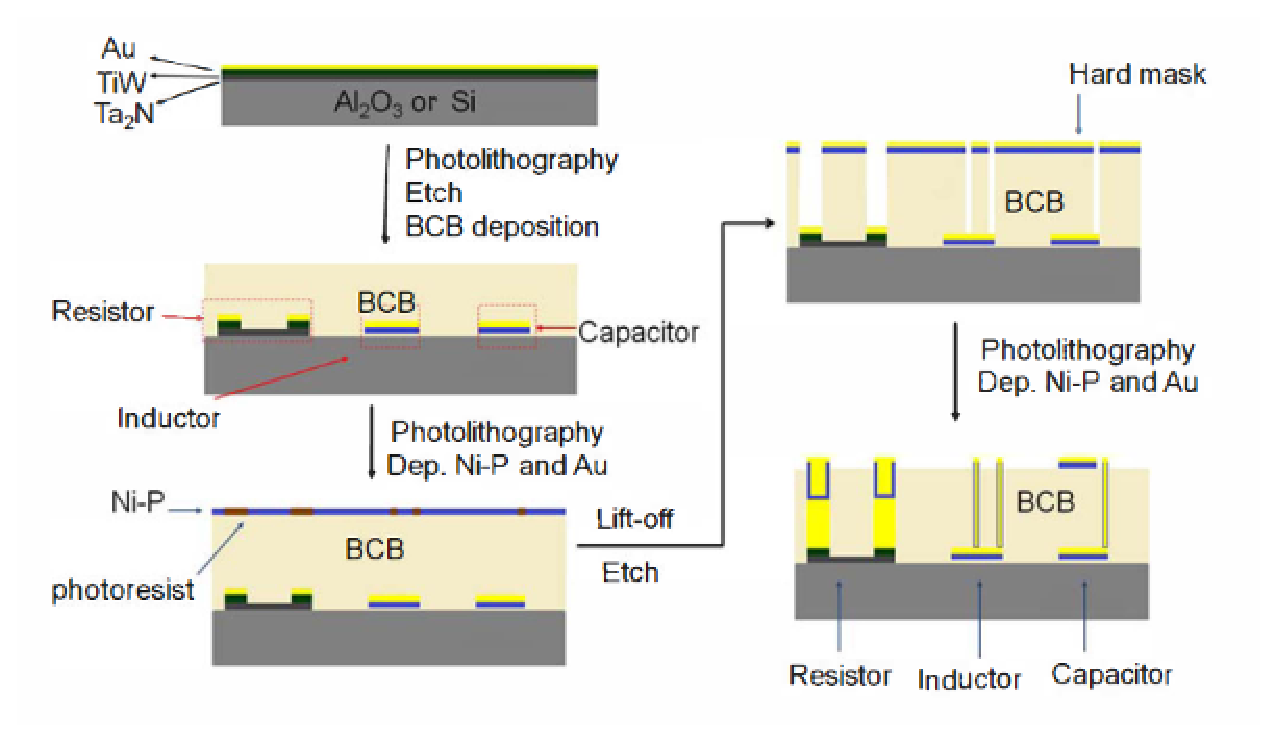
\includegraphics[width=4in, fbox]{Chapter3/3.eps}
	\caption{Schematic of MCM-D packaging.}
	\label{fig:chpt3.3} 
\end{figure}

MCM-D uses thin-film deposition technology to deposit metal materials onto ceramic or silicon or aluminum substrates, lithographing signal lines, power lines, and ground lines, and making multi-layer substrates (up to several dozen layers) in turn. It is mainly used in high-performance products above 500MHz, with a line width and spacing of 10-25mm μm and an aperture of 1050μm, thus having the advantages of high assembly density, short signal channels, small parasitic effects, and low noise, which can significantly improve the high-frequency performance of the system.

MCM-D is the most expensive of several substrates, mainly because the wiring uses a process similar to that used in chip manufacturing. MCM-D forms the interconnected signal lines of the substrate by depositing a thin metal film. Its substrate multilayer wiring process can be planned as a thin film process. If Si is used as the substrate, i.e. MCM-Si, also using Al as the wiring material, the fabrication process is identical to that of the IC chip, with the main difference being the number of layers of wiring. Generally, the metal wiring of a chip does not exceed two layers, whereas the wiring of MCM-D is usually no less than two layers. The ceramic-based MCM-D wiring process is similar to the conventional thin-film circuit manufacturing process. A typical MCM-d substrate fabrication process is shown below.

\begin{figure}[ht]
	\centering
	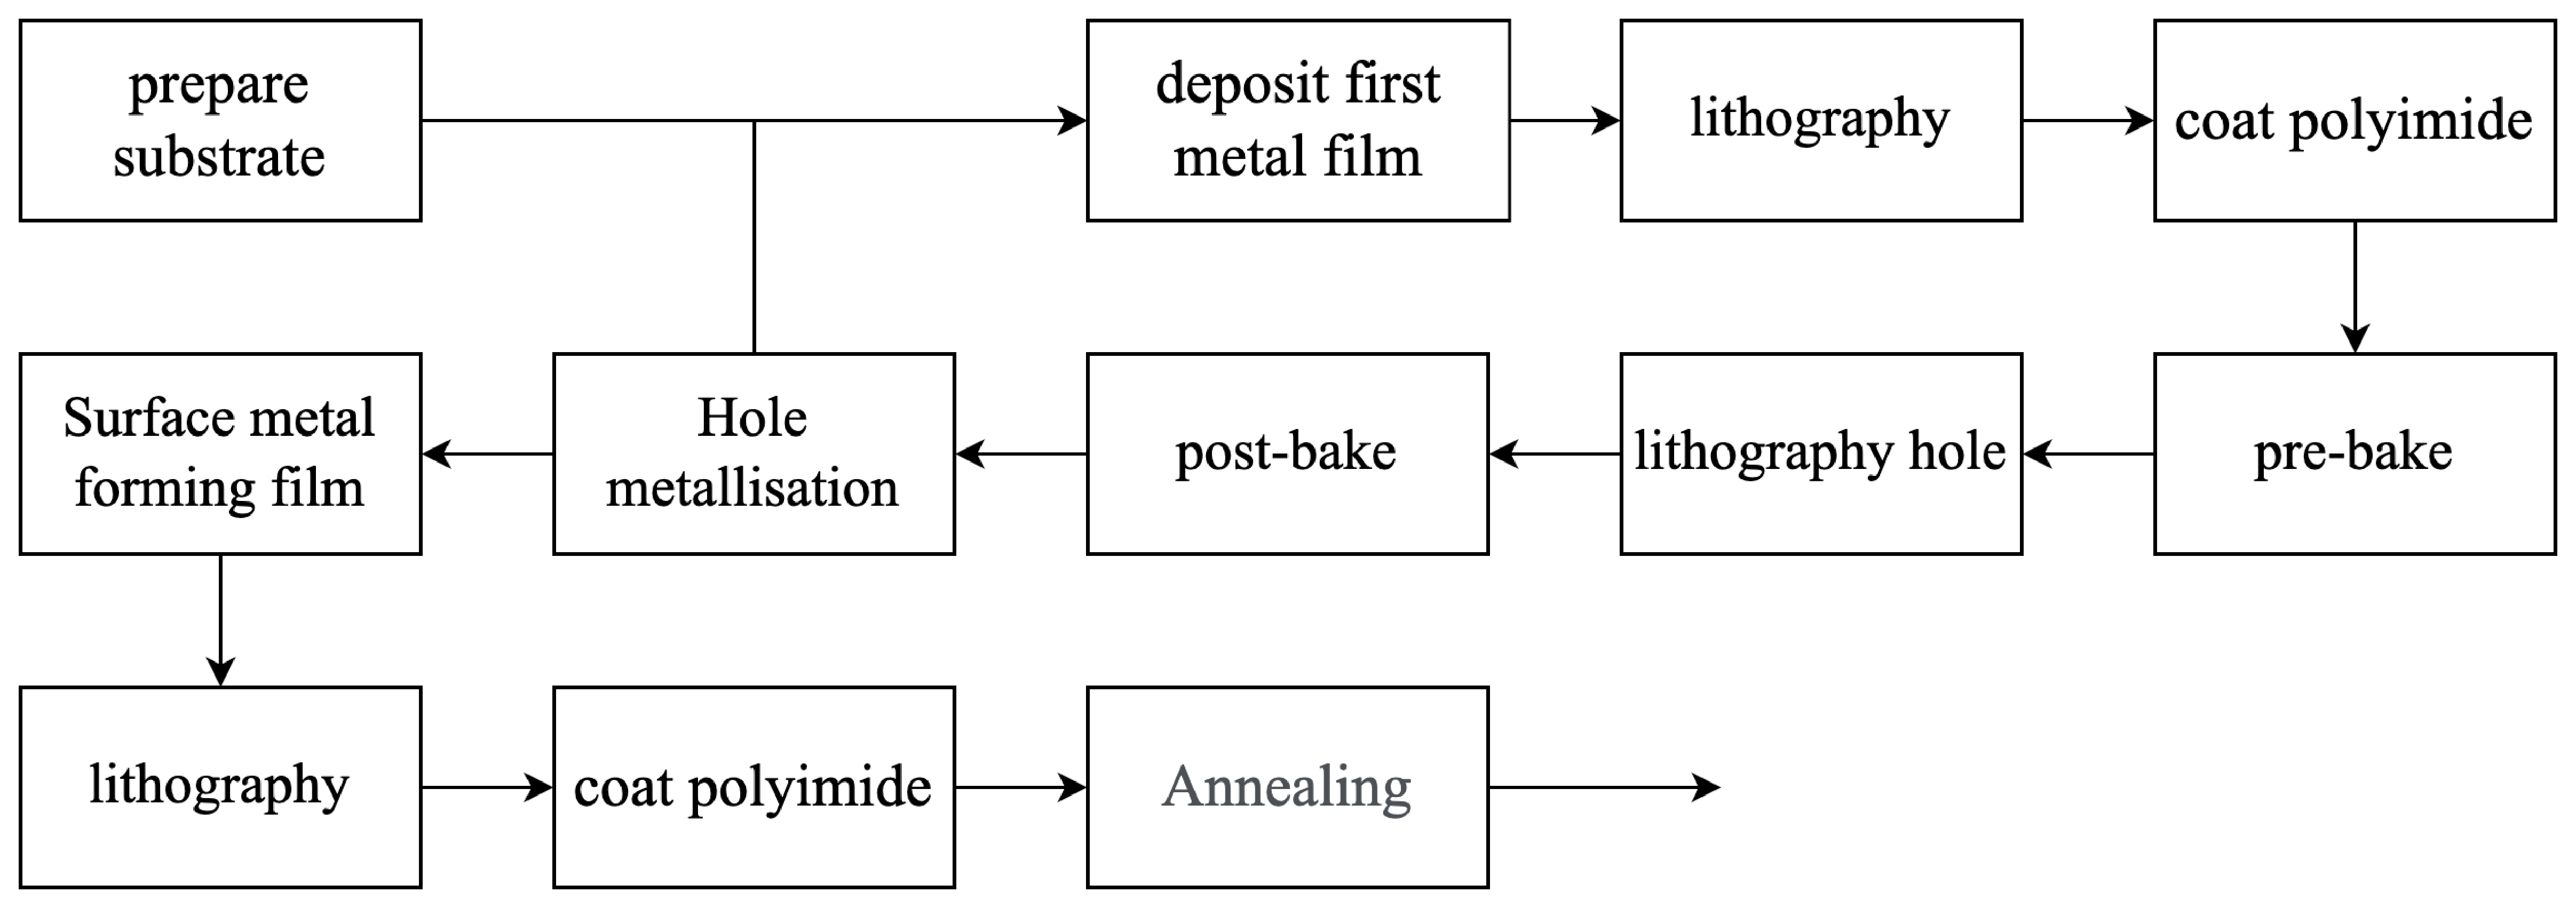
\includegraphics[width=4in, fbox]{Chapter3/4.eps}
	\caption{Work flow of MCM-D packaging.}
	\label{fig:chpt3.4} 
\end{figure}

\section{MCM-PCB}

Because ceramic materials are not easy to sinter and produced, and the functions of ceramic substrates many are very similar to PCB multilayer circuit boards, there are also manufacturers who use PCB multilayer circuit boards as the substrate of MCM. However, the moisture absorption of PCB multilayer circuit boards has always been an obstacle to its use in harsh conditions. Furthermore, coupled with the poor heat resistance of PCB multilayer circuit boards, although new materials and processes, and high-density interconnect (HDI) wiring technology, the cost of the plate is low, the processing is convenient, and it has economies of scale, which can already meet the requirements of environmental standards, it is still difficult to break through the traditional application fields dominated by ceramic substrates for a while.

%=== END OF CHAPTER THREE ===
\end{spacing}
\newpage
